\documentclass{article}

\usepackage{hyperref}
\usepackage{amsmath}
\usepackage{graphicx}
\usepackage{float}

\graphicspath{ {/Users/laralu/Google\ Drive/udacity/projects/projects/capstone/graphs} }

\setlength\parindent{2em}
\setlength{\parskip}{1em}

\begin{document}
\title{ML Engineer Nanodegree Capstone}
\author{Lara Lu}
\maketitle
\section{Definition}
\subsection{Project Overview}
According to Mordor Intelligence, the wine market is value at 287.39 billion USD in 2016, and is forecasted to reach 402 billion by 2022\cite{mordorintelligence}. In the US in 2016, 806.45 million gallons of wine was produced\cite{statistica}.  For a beginner, choosing a good bottle of wine can be difficult as there are usually too many options, whether in a liquor store, the wine aisle in a supermarket or online. Many people like me tend to rely on wine ratings from trusted sources, such as WineEnthusiast, to help make a more informed purchase decision. This process works great except for new wines on the market which don't have many reviews yet. In 2017 there are almost 400 new wineries in the US alone\cite{winebusiness} - it is hard to tell from the myriad of new bottles which ones are gems and which ones to avoid. It would be ideal if there is a way to predict the score of a wine from the information we already know.

\subsection{Problem Statement}
Is it possible to predict the rating of a new wine based on what we know about it? Currently there is a dataset on \href{https://www.kaggle.com/zynicide/wine-reviews/}{Kaggle} that is scraped from WineEnthusiatic.com. It includes all the wine listed on the website, their attributes and a score given by a professional reviewer. I will be utilizing this dataset to try to predict wines' scores based on their attributes.

In particular, I use the available attributes, such as description, location of production, price and variety as input, to predict the wine's score. Since the score is numeric, it is a regression problem.

\subsection{Metrics}
A common metric for regression model is coefficient of determination or $R^2$. $R^2$ measures the proportion of the variance in the dependent variable which is predictable from the independent variable. In other words, how much of the actual data can be explained by prediction. 1.0 means perfect correlation, a constant model always outputting the same output will score 0, and it is possible to get a negative score. The higher the $R^2$ score, the better the model is.

An alternative measure is Mean Squared Error (MSE), which measures how much our predictions deviate, on average, from the actual values. Both can be useful with regression problems, but I choose $R^2$ because it is scaled between 0 and 1 so that it is comparable across different problems, and because it is more easily interpretable.

Here is how to calculate $R^2$ score. Supposed the true scores of each wine (observed data) are marked $y_1$,..., $y_n$(collectively known as $y_i$), and the predicted score of each wine are $f_1$,...,$f_n$.

Define the residuals as $e_i = y_i - f_i$.

If $\bar{y}$ is the mean of the observed data:
$$ \bar{y} = \frac{1}{n} \sum_{i=1}^{n} y_i $$

then the variability of the data can be measured using three sums of squares formulas:
\begin{itemize}
  \item The total sum of squares:
  $$SS_{tot} = \sum\limits_{i}{(y_i - \bar{y})^2}$$
  \item The regression sum of squares:
  $$SS_{reg} = \sum\limits_{i}{(f_i - \bar{y})^2} $$
  \item The sum of squares of residuals:
  $$ SS_{res} = \sum\limits_{i}{(\bar{y} - f_i)^2} = \sum\limits_{i}{e_i^2} $$
\end{itemize}
 
The definition of the coefficient of determination is
$$ R^2 = 1 - \frac{SS_{res}}{SS_{tot}}$$

\section{Analysis}
\subsection{Data Exploration}
The data I use in this project comprises of two datasets pulled at two different time, namely $winemag-data_first150k.csv$ and $winemag-data-130k-v2.csv$ (\href{https://www.kaggle.com/zynicide/wine-reviews/data}{source}). The combined dataset has 280901 rows and 10 columns. I deduplicated the rows on all columns and ended up with 169776 rows. The following is a description of each column.
\begin{itemize}
  \item Points (Integer):
  the number of points WineEnthusiast rated the wine on a scale of 1-100 (though WineEnthusiast only posts reviews for wines that score $>=$80)
  \item Variety (Categorical String):
  the type of grapes used to make the wine (ie Pinot Noir)
  \item Description (Long String):
  a few sentences from a sommelier describing the wine's taste, smell, look, feel, etc.
  \item Country (Categorical String):
  the country that the wine is from
  \item Province (Categorical String):
  the province or state that the wine is from
  \item Region 1 (Categorical String):
  the wine growing area in a province or state (ie Napa)
  \item Region 2 (Categorical String):
  sometimes there are more specific regions specified within a wine growing area (ie Rutherford inside the Napa Valley), but this value can sometimes be blank
  \item Winery (Categorical String):
  the winery that made the wine
  \item Designation (String):
  the vineyard within the winery where the grapes that made the wine are from
  \item Price (Float):
  the cost for a bottle of the wine
\end{itemize}

\subsection{Exploratory Visualization}
In order to gain an overall understanding of the characteristics of the different columns, I use pandas.DataFrame.describe api to summarize the basic statistics (Fig. 1). Country is a categorical column containing 48 unique values. Description is a long corpus with 97821 unique values. Designation is a text field of 30621 distinct values, meaning on average around wines share the same designation. Region 1 has 1236 unique values, whereas the less granular province has 455 unique values, and region 2, which is the least granular, has only 18 unique values. There are 632 unique varieties. There are 14810 wineries, each on average makes 6.6 different wines. The average price for all wines is \$33.66, with standard deviation of \$37.67. The average points is \$87.96, with standard deviation of \$3.22.

\begin{figure}[H]
\caption{Statistics summary}
\centering
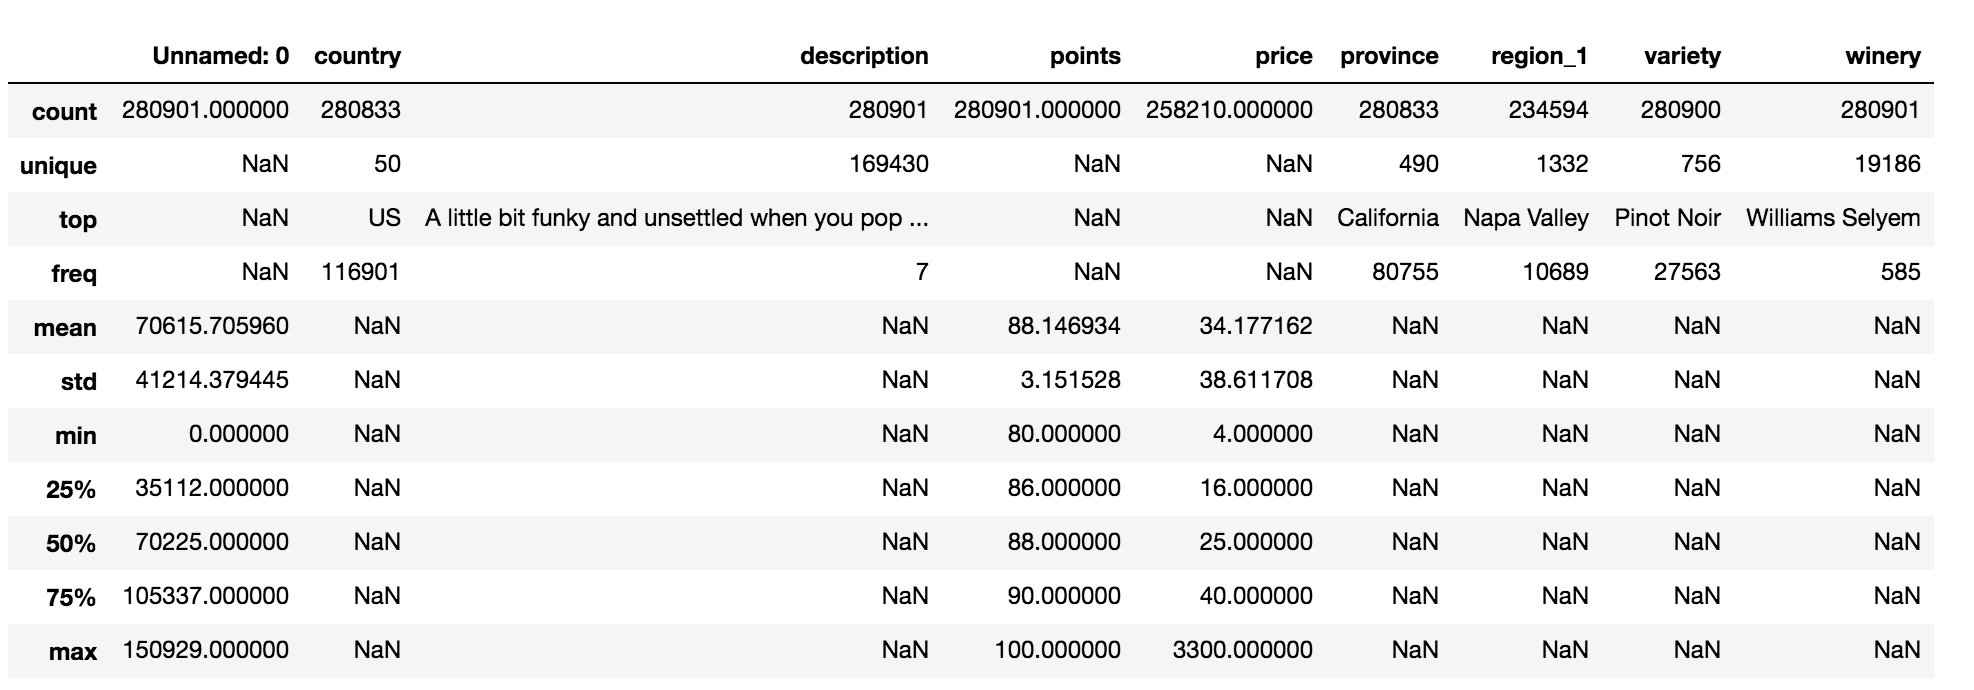
\includegraphics[width=1.2\textwidth]{graphs/data_describe.png}
\end{figure}

I want to deep dive into some of the interesting aspects of data by analyzing individual columns and visualizing the data. Below is the top 10 countries that produce the largest number of distinct wines (Fig 2). US leads the chart, producing over 70000 wines - more than Italy, France and Spain, which follow the list, combined.

\begin{figure}[H]
\caption{Top 10 Wine Producing Countries}
\centering
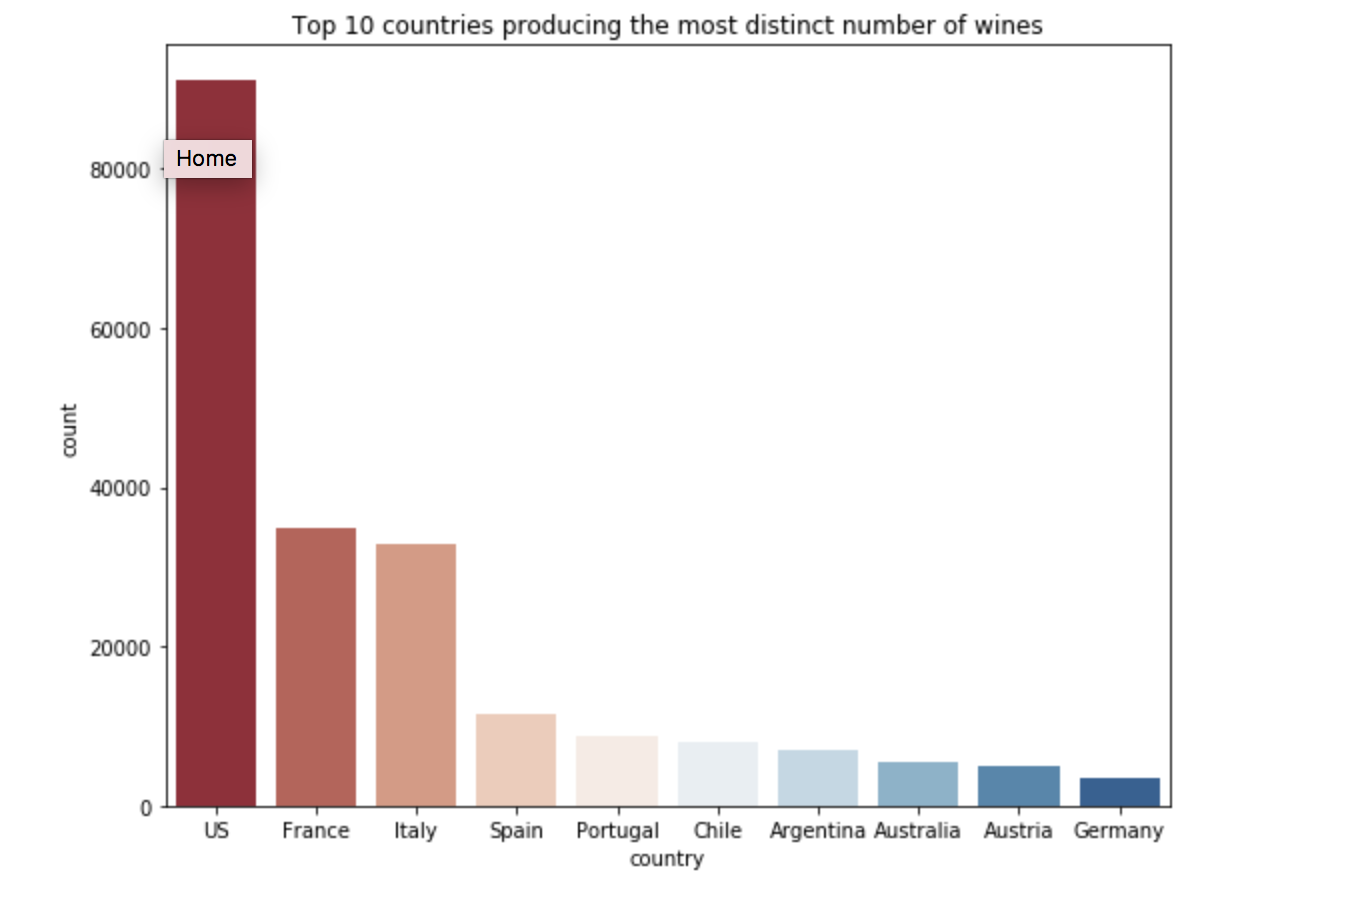
\includegraphics[width=0.85\textwidth]{graphs/top_10_countries}
\end{figure}

Kernal density estimate is a non-parametric way to estimate the probability density function of a random variable. I plotted the kernel density estimate of the price and points of 5000 sampled data points in a 2D graph (Fig. 3). According to the graph, it is the most probable that a randomly chosen wine is priced around \$20, and has points of 87.5. It is unlikely that the price goes below \$10, but it is common to be anywhere under \$50. 
\begin{figure}[H]
\caption{Kernal Density Estimate - Price and Points}
\centering
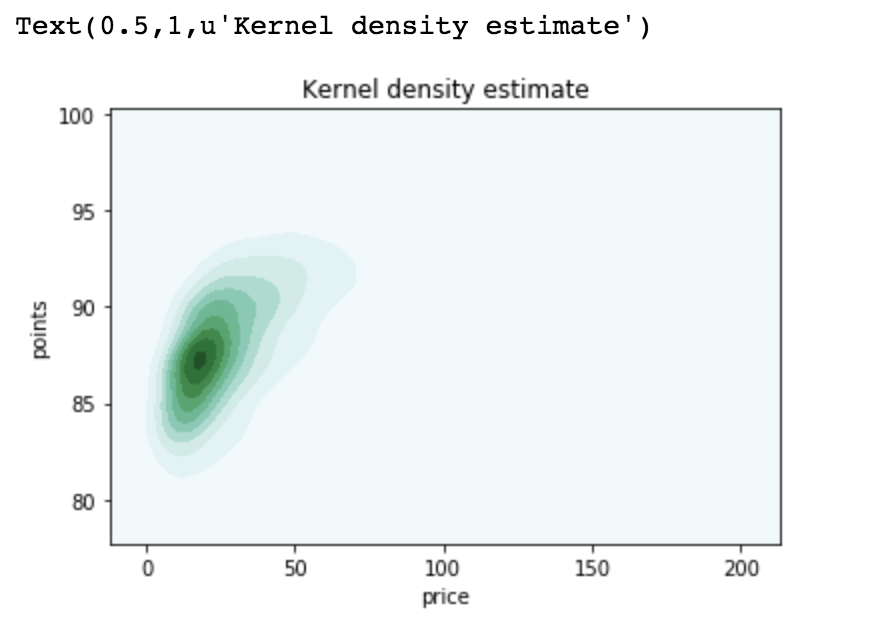
\includegraphics[width=0.8\textwidth]{graphs/kernal_density_estimate}
\end{figure}

Different provinces usually produce wines at different price level. I use box plot to visualize for the top 15 provinces, the distribution of price (Fig. 4). Burgundy, Tuscany, and Piedmont provinces produce wines that are noticeably more expensive than other provinces. The average price of a Tuscan wine is around \$50, the 75th percentile is around \$80. In contrast, on the low end, an average wine produced in Mendoza Province in Argentina only sells for around \$15.

\begin{figure}[H]
\caption{Boxplot of Province and Price}
\centering
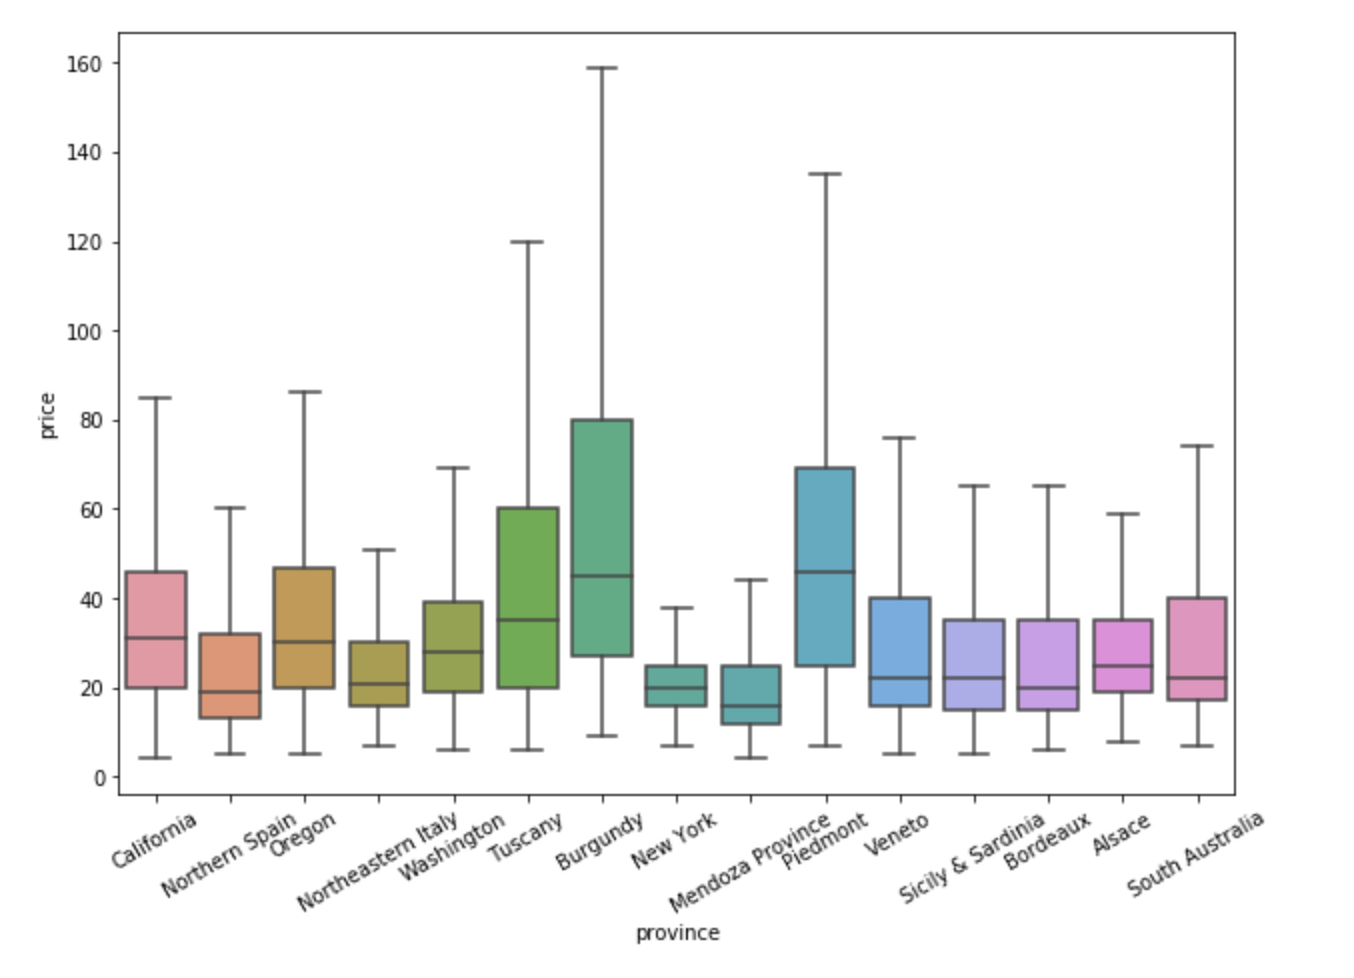
\includegraphics[width=1\textwidth]{graphs/province_price_boxplot}
\end{figure}

\subsection{Algorithms and Techniques}
The key characteristic of the input feature is that it will be sparse. This is because I plan to incorporate wine description, which is a long corpus field, into the feature vector by using tf-idf. Traditional regressors such as random forest does not fit well with sparse data as bagging and suboptimal selection of splits may waste most of the model insight on zero-only areas. I will use a stochastic gradient descent regressor instead, which has shown success on large and sparse data\cite{sklearn_sgd}.

To understand how stochastic gradient descent regressor works, we first need to understand batch gradient descent. Suppose there are m data points, and we have the parameters $\theta$, the object function $J(\theta)$ will have the form:
$$ J(\theta)  = \sum_{i=1}^{m} J_{i}(\theta) $$
where $J_{i}$ is associated with the $i^{th}$ observation in the dataset. In batch gradient descent, we start with an initial $\theta$ and repeatedly perform the following update to $\theta$:
$$\theta := \theta-\eta \sum_{i=1}^{m}\nabla J_{i}(\theta)$$
where $\eta$ is the learning rate. In order to make a single update, we need to pass through the entire dataset.

Batch gradient descent is guaranteed to converge to global minimum for convex error surfaces and a local minimum for non-convex surfaces. The problem with batch gradient descent is that when we pass large datasets the calculation of $\nabla J(\theta)$ is expensive. 

Stochastic gradient descent overcomes the problem by updating $\theta$ every time a data point is passed. The update takes the form:
$$ \theta := \theta - \alpha \nabla_{\theta} J_{i}(\theta) $$.

SGD is computationally cheaper, but results in a larger variance of the loss function in comparison with batch gradient descent.

\subsection{Benchmark}
I have not found any existing solution to the regression problem I am trying to solve for the wine dataset online. For the sake of comparison, I will use a use a linear regression model on the same features as benchmark. Linear regression tries to find a weight for each feature and an intercept so that the residual sum of squared error is minimized. I will measure the performance of the benchmark model using $R^2$ as well for fair comparison against that of my model.

\section{Methodology}
\subsection{Data Preprocessing}
As described in Data Exploration, the raw data columns contain string or numeric values. Some columns are categorical and others are not. The goal of data preprocessing is to convert each row into a vector that the machine learning model could accept. In this section, I will select the columns that I think are most important, vectorize them individually and concatenate them into one vector.

First, I will handpick the columns that I think will be most valuable to our ML problem. In terms of relevancy, I think all columns are key aspects of wine that can be useful for predicting the score. I want to exclude any column with too many missing values. An analysis on the density of columns shows that only $region\_2$'s missing value percentage is 60.3\% and all other columns' in the single digit. I therefore decide to drop $region_2$. In the remaining columns, $country$, $province$, $region\_1$ and $winery$ are all categorical values related to the location of the winery. I decide to keep $province$ as its number of distinct values is reasonable (490). It is not as coarse as $country$, which only has 50 distinct values, and not as many as $region\_1$ (1332) or $winery$ (19186). This leaves us with 4 final columns: $description$, $province$, $price$ and $variety$.

$Description$ is the most challenging and critical column to preprocess. On the one hand, descriptions are written by wine expert to describe each wine, and therefore should contain rich information about the wine's quality and value. On the other hand, it typically contains many words and can be difficult to vectorize in a way that preserves the features. A common way to preprocess a corpus is bag of words. Corpus is first tokenized and normalized. The resulting matrix's columns correspond to each token, and each row corresponds to a sample with values being the frequency that the token appeared the in sample's document. The drawback of this method is that more common words, such as ``wine" in our case, will have a high frequency and high values, but they typically carry little meaning. Tf-idf helps the issue by discounting the frequency by an idf component that denotes the popularity of the term across all documents. I will use Tf-idf to vectorize description.

$Province$ and $variety$ are both categorical columns. I use one hot encoder to transform them into vectors where each column corresponds to a category and the value at each column is a binary that denotes if the row belongs to the category.

$Price$ is a numeric value field that can be directly used. The prices of wines have a large range, from $4 to $3300. However, most wines are between \$20 to \$60, with a mean of \$34.17 and standard deviation of \$38.6. I will use a scaler to scale it to zero mean and unit variance.

After vectorizing the four individual columns, I concatenate them into a single feature vector.

\subsection{Implementation}
With the preprocessed dataset being rows of feature vector and label (score), I split it into training and testing set. As explained in Algorithms and Techniques, I will use Stochastic Gradient Descent regressor as the model. Sklearn provides SGDRegressor under the linear\_model library. I specify the following parameters when constructing the regressor. I set $max_iter$, which is the maximum number of passes over the training data, also known as epoch, to 50. Because in our case the control for stopping criteria (tol) is not set, the model will be trained exactly for 50 iterations. I set learning rate to be constant, which means it will use the same $\eta$ (which defaults to 0.01) to perform parameter update in each iteration. 

To train the model, I call $fit$ on the constructed SGDRegresssor on training features and labels. The regressor will update parameters in every iteration in order to minimize the loss function on the training data. In our case, the parameters are the weights of each feature column (hypothesis is linear), and the loss function is squared mean error (default). In each epoch, we pass each individual training data's feature to make a prediction. The parameters are then updated by the derivative of the loss function scaled by the learning rate $\eta$. In each epoch, we go through all the training samples individually for weight update. The weights will be closer and closer to the local best setting (local maxima) to minimize training errors as we run more epochs.

The test data is not used at all during the training phase, and will used exclusively for testing (will discuss more in Results). The reason is two folds. First, in some cases trained models can overfit or underfit training data. If simply judge a model's merits by its performance on training data, an overfit model can perform well but will not generalize to real world data. We need to separate out a small testing set that should reflect the real world against which the model should be tested on. Second, as I will explore in the next section, models can be refined through hyper parameter optimization. The process of optimization has a favorable bias towards the training data. In order to validate that the winning hyper parameter can generalize properly, we should run a sanity check on the test set.


\subsection{Refinement}
In Implementation, I manually picked the hyper parameters that are associated with the estimator. However, there are many possible combinations of hyper parameters and some might result in training a model that is better than others. I want to try to refine the model by trying different combinations of the parameters to the estimators.

In Sklearn, the class $GridSearchCV$ is designed for the exact purpose of hyper parameter search. I create a grid keyed by four parameters to constructing $SGDRegressor$, namely $max\_iter$, $penalty$, $learning\_rate$, and $power\_t$. For each parameter, I provide a list of values that I am interested in trying. I have explained $max\_iter$ and $learning\_rate$ in the previous section. $penalty$ refers to the regularization term, and $power\_t$, when $learning\_rate$ is set to inverse scaling, controls the exponent for the inverse scaling. Below are the candidate values for each hyper parameter:

\begin{itemize}
  \item max\_iter:
  20, 50, 100
  \item penalty:
  L1, L2
  \item learning\_rate:
  constant, optimal, inverse scaling
  \item power\_t:
  0.15, 0.25, 0.35
\end{itemize}

$GridSearchCV$ will use each combination of parameter and value (54 combinations in total) to train a SGDRegressor model using the training set, and search for the best estimator based on the R2 score on the training set.

\section{Results}
\subsection{Model Evaluation and Validation}
The best estimator selected by $GridSearchCV$ has R2 score of 0.6908 on the test set, which means that 69.08\% of the predicted score for the test set can be explained by the actual scores. As mentioned in Metrics, random guess will result in an R2 score of 0, and perfect correlation will result in an R2 score of 1. Given the sparsity of the data and the small number of training data, I think 0.6908 is a decent score.

Here are the hyper parameters values that $GridSearchCV$ has selected:
 \begin{itemize}
  \item max\_iter:
  50
  \item penalty:
  L2
  \item learning\_rate:
  constant
  \item power\_t:
  0.15 (does not matter since learning rate is not inverse scaling)
\end{itemize}

\subsection{Justification}
For benchmark, I trained Linear Regression model on the same training set. The R2 score on the test set is 0.6609. It is 4.34\% lower than the SGD Regressor. The different might not seem significant on the first sight. However, it seems like a consistent difference even if I try splitting trainand test set differently. In particular, I did an experiment to split train and test sets using 10 different random seeds, and train SGD Regressor 10 times using the different splits. The results are very consistent. The average R2 score is 0.6806 with standard deviation of only 0.0025. Therefore, I conclude with confidence that SGD Regressor is better in terms of predicting wine scores than Linear Regressor.

Another aspect that we should not overlook is speed. Because of the way SGD updates parameters once per sample, it is much faster to train compared to linear regression, where the coefficient and intercept calculation requires a lot more CPU labor. The speed advantage of SGD is especially evident when sample size is large and features are sparse. On average, the SGD Regressors I trained took 5.9 seconds each to train. In comparison, training a Linear Regressor took 101.1 seconds - a 17 times difference!

\section{Conclusion}
\subsection{Free-Form Visualization}
I have trusted the regressors to assign weights appropriately for the input vector based on the training data, and based on our metric ($R^2$ score), I think it has done a good job. To manually verify it, I visualized the top weighted terms in description and the bottom ones from both the winning SGD Regressor and the benchmark Linear Regressor.

To my pleasant surprise, the result of SGD Regressor (Fig. 5) made a lot of human sense. The words associated with the most positive weights include ``gorgeous" (+6.259), ``beautiful" (+5.638), ``long" (+5.356), ``impressive" (+4.902), and ``complex" (+4.855). On the negative side, we have ``lacks" (-5.333), ``vegetal" (-4.473), ``sugary" (-4.297), ``watery" (-4.151), and ``dull" (-3.864). I am amazed that the model, simply by updating parameters using a mathematical formula with training data, is able to learn the deep connotations of English words for the wine domain without any prior domain knowledge.

The weights from the Linear Regression model is less ideal. As shown in Fig. 6, the top and bottom weighted words are mostly rare words or words without clear positive or negative meanings, and the absolute values of the weights are significantly bigger than that from SGD Regressor's case. This is likely due to Linear Regression models' susceptibility to outliers and its tendency to model noise when feature dimensionality is large.

\begin{figure}[H]
\caption{Importance of description token - SGD Regressor}
\centering
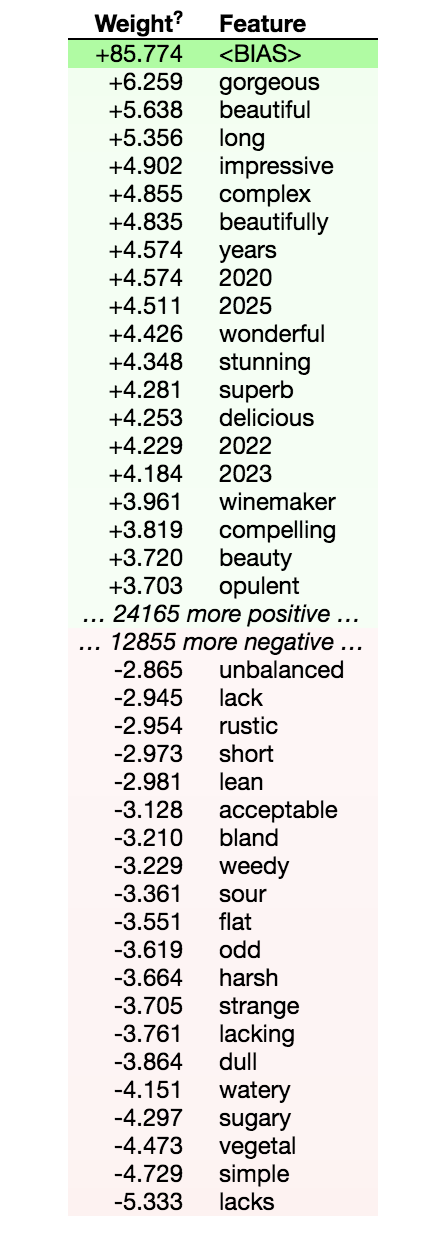
\includegraphics[width=0.4\textwidth]{graphs/sgd_token_weights}
\end{figure}

\begin{figure}[H]
\caption{Importance of description token - Linear Regressor}
\centering
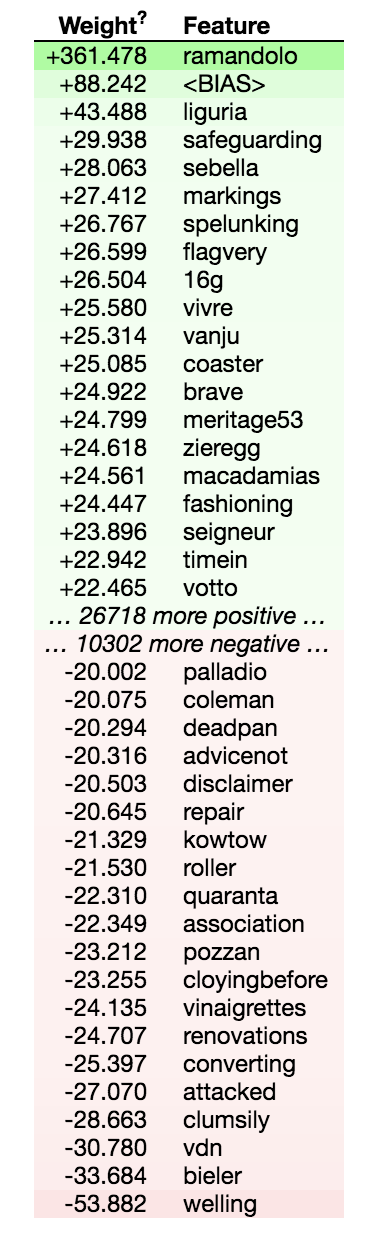
\includegraphics[width=0.35\textwidth]{graphs/lr_token_weights}
\end{figure}

\subsection{Reflection}
The value of wine is a very subjective matter. Even my closest friends have dramatically different taste in wine than I do. It is amazing that through machine learning, we are able to predict the score of a wine relatively closely to a human expert based on the information we have.

My end-to-end solution consists of seven parts: data collection, feature selection, feature engineering/data preprocessing, train test split, model training, hyper parameter optimization and benchmark validation. Among all the parts, I find feature engineering/data preprocessing the most challenging. It is the part where I, as an ML engineer, have the most freedom to decide how to extract the essence of the data, but it also requires acute analysis on the underlying properties of the data, and the knowledge of what techniques to apply based on the properties.

Another equally challenging part is feature selection. I did not spend too much time on it and simply hand selected the columns that I think will be useful based on their semantic meaning and properties such as sparsity. More scientific approaches can be taken to select the most useful set of features. Filtering is the faster approach where we analyze all the features and narrow them down prior to sending them to the learning algorithm. A commonly used method is Principal Component Analysis. Wrapping is the more time consuming way of relying the learning algorithm to decide to best subset of features. By optimizing feature subset for minimizing error on the labels, the second approach will theoretically select more useful features.

\subsection{Improvement}
If I have more time on the project, I would try to improve on the follow three aspects. First, I would like to dive deeper into the details of tf-idf. I would like to know at the end of training, which words have highest weight for driving score up, and which words are deemed indicators of poor wine. I would like to work backwards from there, try to understand if the weights make sense, and if not in some cases, root cause the problem and potentially solve it using specific NLU techniques for preprocessing.

Second, I would like to understand if the training sample is large enough. This can be easily done by using different sizes of the current training set to train the model, and plot the score on test set for different sizes. If the line plateaus after a certain point, it indicates the dataset is large enough. Otherwise, I would like to scrape more data to train a better model, especially because SGD models tend to benefit  from large amount of data.

Third, with larger amount of data, I'd like to experiment with deeper neural network. Our current model is essentially a single layer perceptron. Deeper networks have shown great success at automatically finding patterns that are important to the problem without human assistance. Neurons on different levels represent different abstraction oI meanings that can be concrete or vague to human. I am curious to know if a deeper neural network would be able to extract important meanings by the combinations of words from description. Of course, this might take more than a multilayer perceptron, as it does not know the relationship between input features (words). A convolutional network might be a good alternative Deep neural network also has significantly more parameters, which requires exponentially more training data because of the curse of dimensionality. We are lucky to live in the age of Big Data, having our fingertips on vast amount of assets that unlock the power of Machine Learning. But the volume is not limitless, and the differentiator will always likely be the human intelligence that goes into creating solutions that maximize the use of the data.

\begin{thebibliography}{9}
 
\bibitem{mordorintelligence}
Wine production in the United States and in California from 2006 to 2016 (in million gallons)*,
\\\texttt{https://www.statista.com/statistics/259493/wine-production-in-the-us-and-california/}

\bibitem{statistica}
Mordor intelligence: Global Wine Market - Growth, Trends and Forecasts (2017 - 2022),
\\\texttt{https://www.mordorintelligence.com/industry-reports/wine-market}

\bibitem{winebusiness}
Wine Business Monthly - Number of United States Wineries Reaches 9,091,
\\\texttt{https://www.winebusiness.com/wbm/?go=getArticleSignIn\&dataId=179530}

\bibitem{sklearn_sgd}
Sklearn SGDRegressor Documentation,
\\\texttt{http://scikit-learn.org/stable/modules/sgd.html\#regression}

\end{thebibliography}

\end{document}